\section{ResNet 1D Implementation}

This section walks through the concrete PyTorch implementation of the 1D Residual Network adapted to the anomaly classification task. All paths below are relative to the \texttt{architectures/} directory.

\subsection{Architecture (\texttt{saved\_models/resNet.py})}

Each stage is a \texttt{\_ResBlock}: three consecutive Conv-GN-ReLU layers whose output is summed with a shortcut connection (a 1$\times$1 projection when the channel count changes, otherwise identity). The trailing ReLU is dropped from the body so the residual sum happens \emph{before} the final non-linearity. The full network stacks three such blocks with intermediate \texttt{MaxPool1d(2)} downsampling and feeds an \texttt{AdaptiveAvgPool1d(4)} head identical to the 1D-CNN's, for a fair comparison.

\textbf{Adaptations versus a textbook ResNet1D:}
\begin{itemize}
    \item Channel widths reduced from $(64,128,128)$ to $(16,32,64)$ to keep the parameter count tractable.
    \item \texttt{AdaptiveAvgPool1d(4)} instead of pooling to a single bin, to preserve shape topography.
    \item \texttt{GroupNorm(8)} replaces \texttt{BatchNorm1d} everywhere: it carries no running statistics, so train and eval normalize identically and validation-loss spikes disappear.
    \item A larger first-stage kernel set $(15,9,5)$ to enlarge the receptive field at the input.
    \item Same dense head as the 1D-CNN (Linear $\rightarrow$ ReLU $\rightarrow$ Dropout $\rightarrow$ Linear).
\end{itemize}

\begin{lstlisting}[language=Python]
class _ResBlock(nn.Module):
    def __init__(self, in_ch, out_ch, kernels=(7, 5, 3)):
        super().__init__()
        layers, prev = [], in_ch
        for k in kernels:
            layers += [
                nn.Conv1d(prev, out_ch, k, padding=k//2, bias=False),
                nn.GroupNorm(min(8, out_ch), out_ch),
                nn.ReLU(inplace=True)]
            prev = out_ch
        layers = layers[:-1]  # drop trailing ReLU, fuse after residual
        self.body = nn.Sequential(*layers)
        self.shortcut = (
            nn.Sequential(nn.Conv1d(in_ch, out_ch, 1, bias=False),
                          nn.GroupNorm(min(8, out_ch), out_ch))
            if in_ch != out_ch else nn.Identity())
        self.act = nn.ReLU(inplace=True)

    def forward(self, x):
        return self.act(self.body(x) + self.shortcut(x))


class ResNet1D(nn.Module):
    def __init__(self, num_classes, in_channels=1,
                 widths=(16, 32, 64), dropout=0.3):
        super().__init__()
        c1, c2, c3 = widths
        self.block1 = _ResBlock(in_channels, c1, kernels=(15, 9, 5))
        self.pool1  = nn.MaxPool1d(2)
        self.block2 = _ResBlock(c1, c2, kernels=(7, 5, 3))
        self.pool2  = nn.MaxPool1d(2)
        self.block3 = _ResBlock(c2, c3, kernels=(7, 5, 3))
        self.gap = nn.AdaptiveAvgPool1d(4)
        self.classifier = nn.Sequential(
            nn.Flatten(), nn.Dropout(dropout),
            nn.Linear(c3 * 4, 32), nn.ReLU(),
            nn.Dropout(0.2), nn.Linear(32, num_classes))
\end{lstlisting}

\subsection{Training Configuration}

All three architectures in this project share the exact same training loop (\texttt{train.py}) and dataset split, so that any difference in evaluation reflects the model itself and not the training recipe.

\begin{itemize}
    \item \textbf{Dataset:} 312{,}470 windows of length 512 (199{,}988 train / 49{,}997 validation / 62{,}485 test), 7 classes, temporal split (no leakage across train/val/test).
    \item \textbf{Optimizer / loss:} Adam, learning rate $10^{-3}$, weighted cross-entropy (class weights inversely proportional to frequency).
    \item \textbf{Scheduler:} \texttt{ReduceLROnPlateau} (patience 2, factor 0.5) monitored on validation loss.
    \item \textbf{Regularization:} dropout 0.3 in the dense head and \texttt{GroupNorm(8)} throughout; early stopping with patience 10 and min-delta 0.005.
    \item \textbf{Batch size:} 128, max 35 epochs, sliding-window stride 32 during training.
    \item \textbf{Total parameters:} 74{,}631 trainable.
\end{itemize}

\subsection{Training Results}

The residual pathways visibly accelerate convergence: validation Macro F1 already exceeds the 1D-CNN's final value after the first epoch. The scheduler triggers twice (epoch 22 and 26), refining the optimum.

\begin{figure}[H]
    \centering
    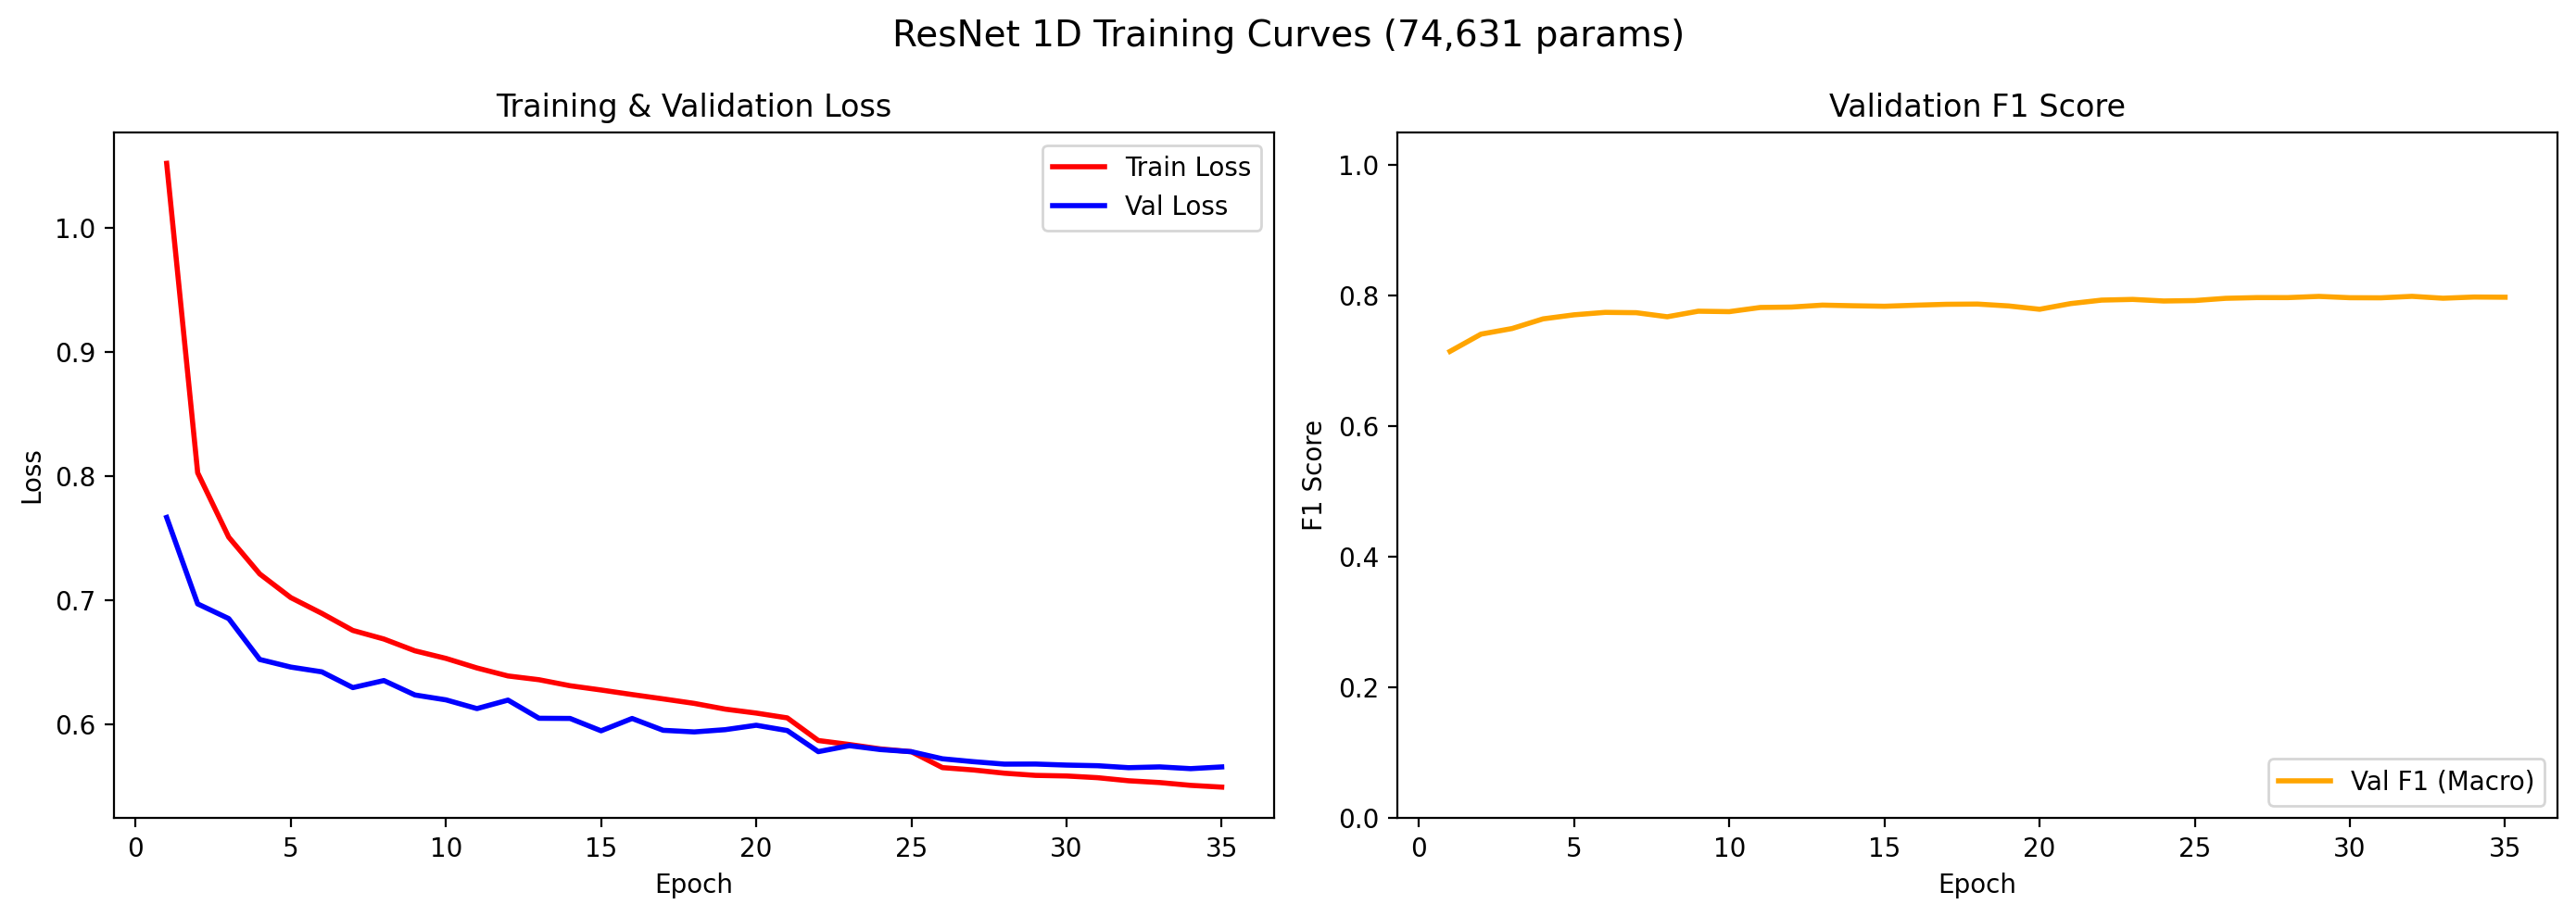
\includegraphics[width=0.85\textwidth]{media/resnet_training_curves.png}
    \caption{ResNet 1D training and validation curves.}
\end{figure}

\begin{itemize}
    \item \textbf{Training duration:} 10:02 on an RTX 5060 Laptop GPU.
    \item \textbf{Best validation loss:} 0.5675 (epoch 30), validation Macro F1 0.7987.
    \item \textbf{Test loss / accuracy:} 0.6210 / \textbf{80.7\%} (50{,}405 / 62{,}485).
    \item \textbf{Per-class accuracy:} Normal Background 94.2\%, bell 77.9\%, bell\_sq 71.3\%, fast\_ascend 73.7\%, fast\_descend 74.1\%, M 76.5\%, square 74.0\%.
\end{itemize}

\subsection{Event-Level Inference Results}

The trained model is evaluated end-to-end on a 100{,}000-point continuous segment by \texttt{visualize\_inference.py}, with a sliding window of stride 10 and per-step probability averaging.

\begin{figure}[H]
    \centering
    \begin{minipage}[c]{0.48\textwidth}
        \centering
        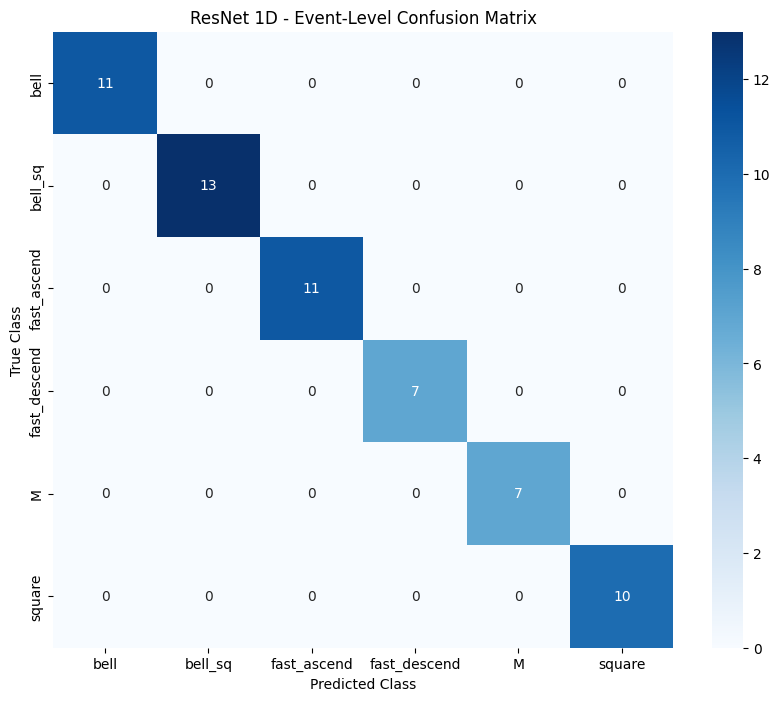
\includegraphics[width=\linewidth]{media/resnet_confusion_matrix.png}
    \end{minipage}\hfill
    \begin{minipage}[c]{0.48\textwidth}
        \centering
        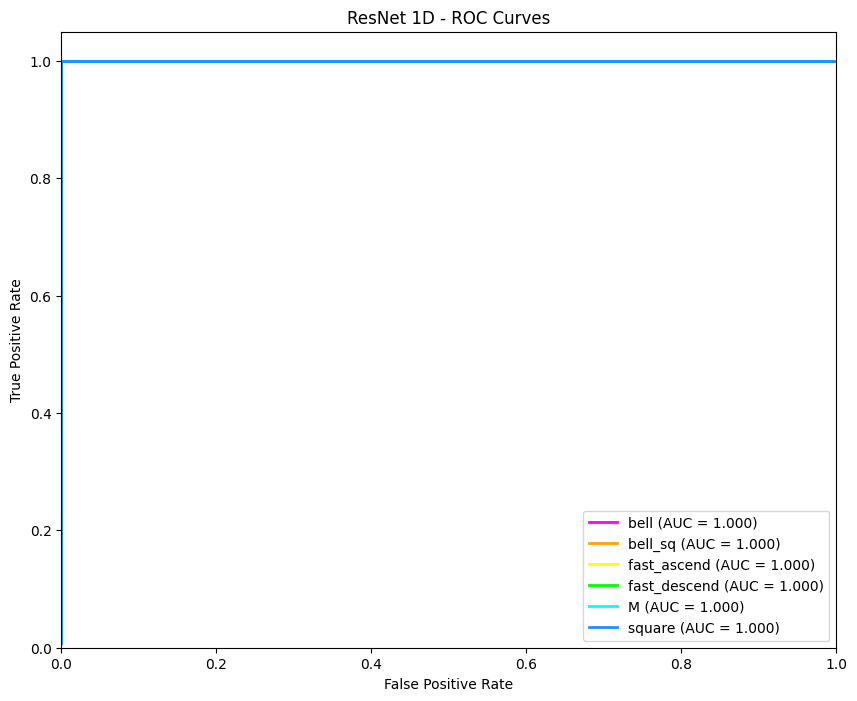
\includegraphics[width=\linewidth]{media/resnet_roc_curves.png}
    \end{minipage}
    \caption{ResNet 1D event-level confusion matrix (left) and per-class ROC curves (right).}
\end{figure}

\begin{figure}[H]
    \centering
    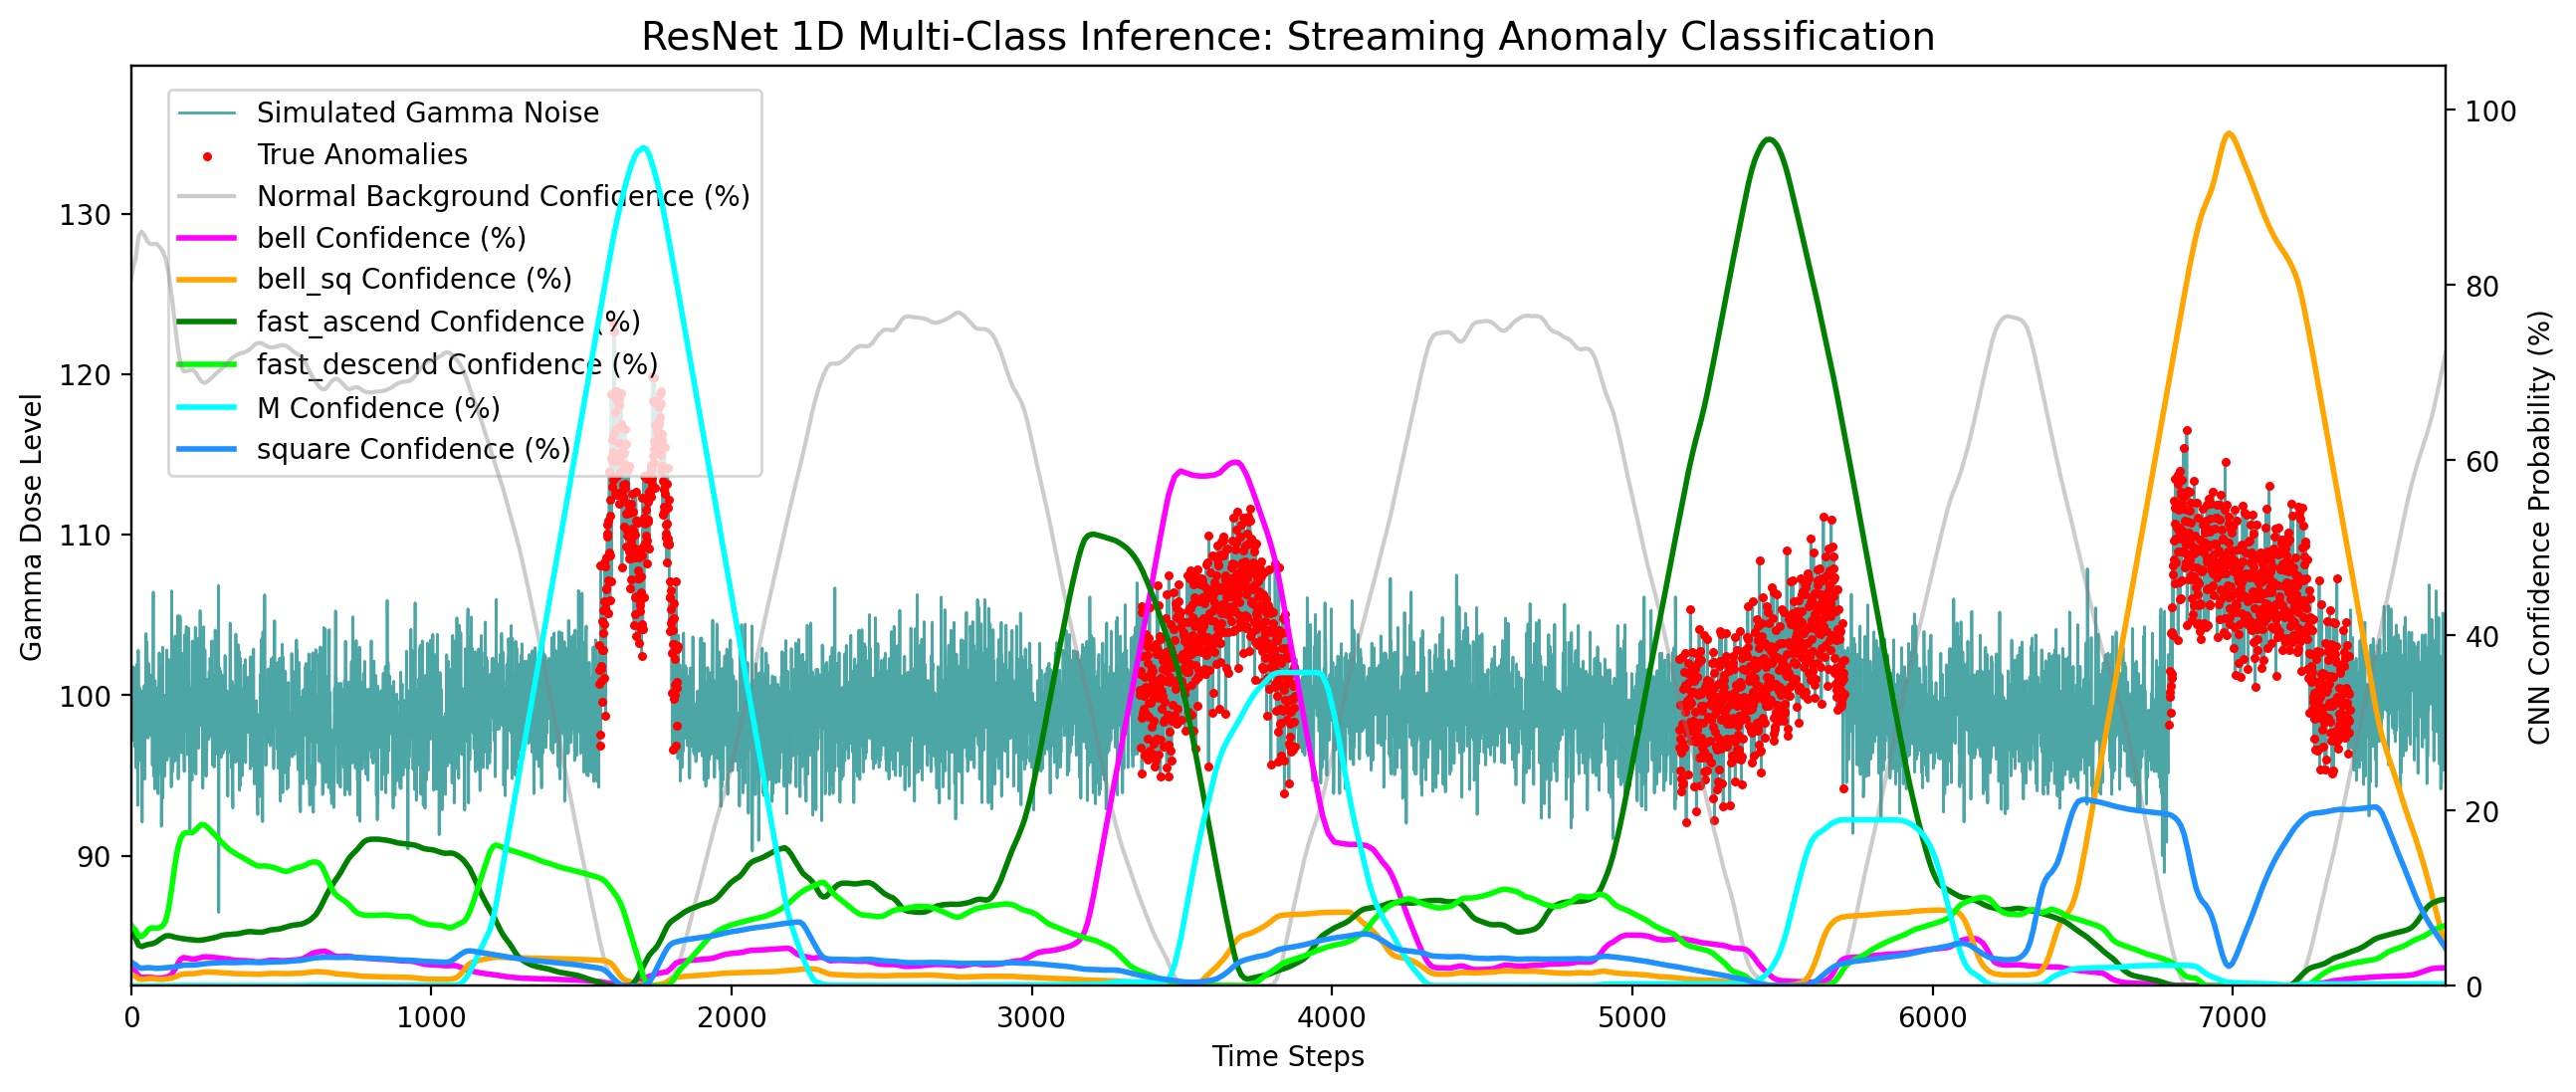
\includegraphics[width=0.95\textwidth]{media/resnet_cnn_inference_visualization.png}
    \caption{ResNet 1D sliding-window inference over a synthetic segment.}
\end{figure}

\begin{itemize}
    \item \textbf{Events:} 59 ground-truth events in the segment.
    \item \textbf{Detection rate (any anomaly):} 59 / 59 = \textbf{100.0\%}.
    \item \textbf{Exact classification:} 59 / 59 = \textbf{100.0\%} (flawless).
    \item \textbf{Mean event confidence:} 70.6\%.
    \item \textbf{Macro precision / recall / F1:} 1.0000 / 1.0000 / 1.0000.
    \item \textbf{Throughput:} 9{,}949 windows in 0.69\,s (\textasciitilde14{,}232 windows/s), massively accelerated by batched inference.
\end{itemize}

\subsection{Robustness Test}

\texttt{robustness\_test.py} sweeps two stressors independently: the standard deviation of the OU background noise and the geometric deformation of injected anomaly templates (see \texttt{data-gen}). For each multiplier, 50 events are regenerated and the model is re-evaluated event-level.

\begin{figure}[H]
    \centering
    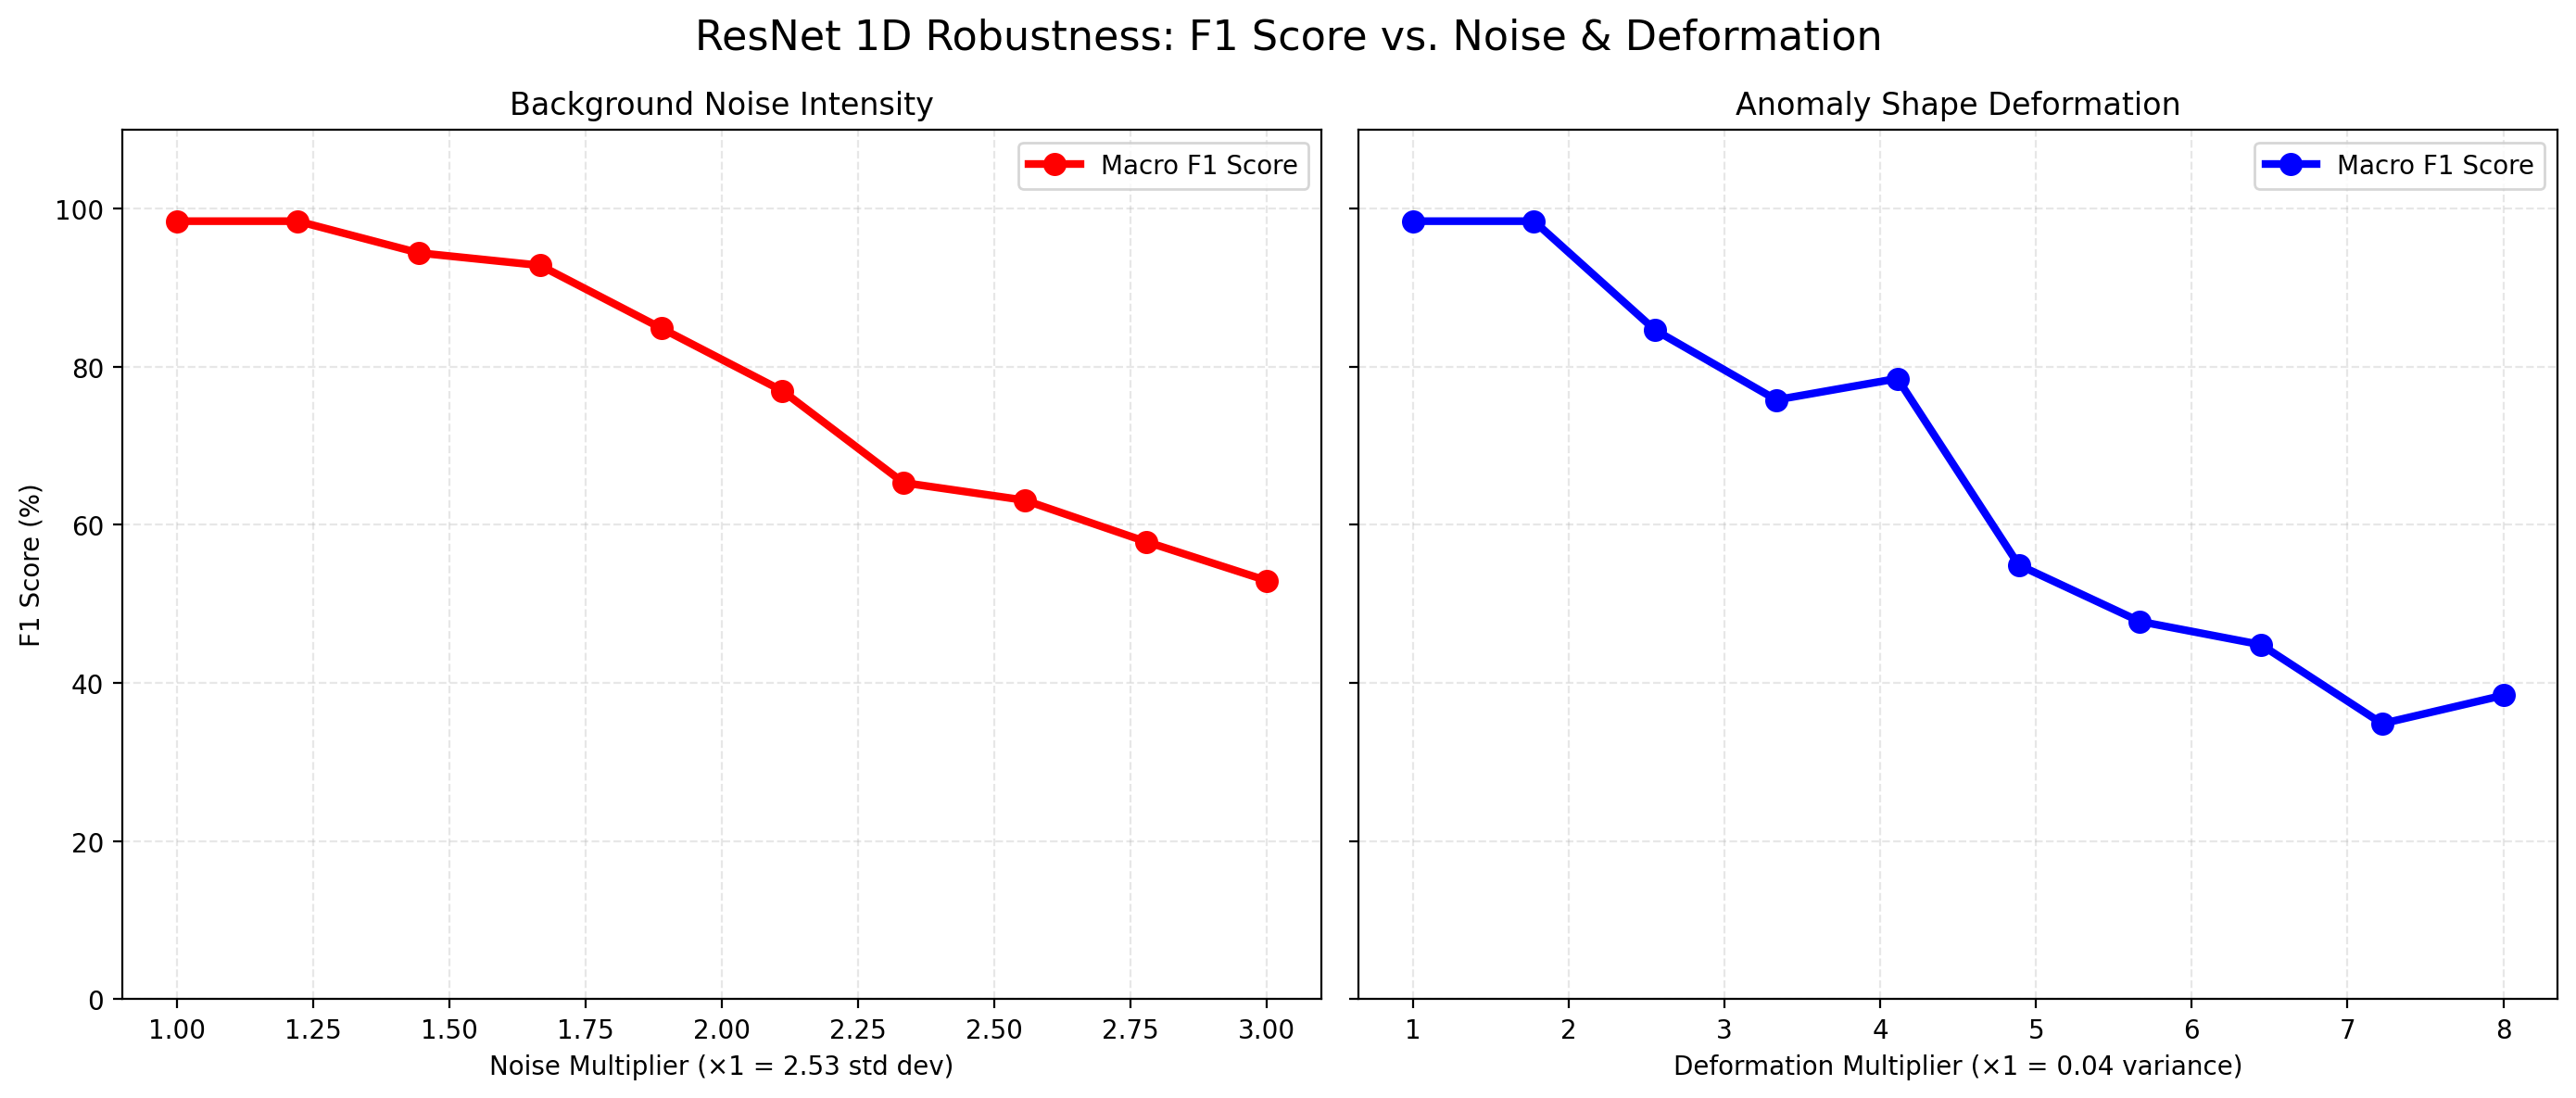
\includegraphics[width=0.85\textwidth]{media/resnet_robustness_test.png}
    \caption{ResNet 1D robustness under increasing background noise (left) and template deformation (right).}
\end{figure}

\begin{itemize}
    \item \textbf{Noise breakdown:} Macro F1 remains at >50\% across the entire sweep up to $3.0\times$ baseline noise --- the model never breaks down within the tested range.
    \item \textbf{Deformation breakdown:} Macro F1 first drops below 50\% at multiplier \(\approx 5.7\times\) the baseline deformation variance.
\end{itemize}

The residual connections substantially improve noise robustness compared with the plain 1D-CNN: by giving every block direct access to lower-level features, the network can rely on coarse-scale evidence when fine-grained features are buried in noise.
